\documentclass{article}
\usepackage[utf8]{inputenc}
\usepackage{graphicx}
\title{My experience as a student of the department of CSE, RU}
\author{Md Rakib Hossain\\2010576143}
\date{December 2022}

\begin{document}
\maketitle
\section{Introduction}
Hello, I am Md Rakib Hossain. I was born in Ullapara, Sirajgang under Rajshahi division in 2001. In figure-\ref{fig:a}, I have shown my picture.
\begin{figure}[h]
    \centering
    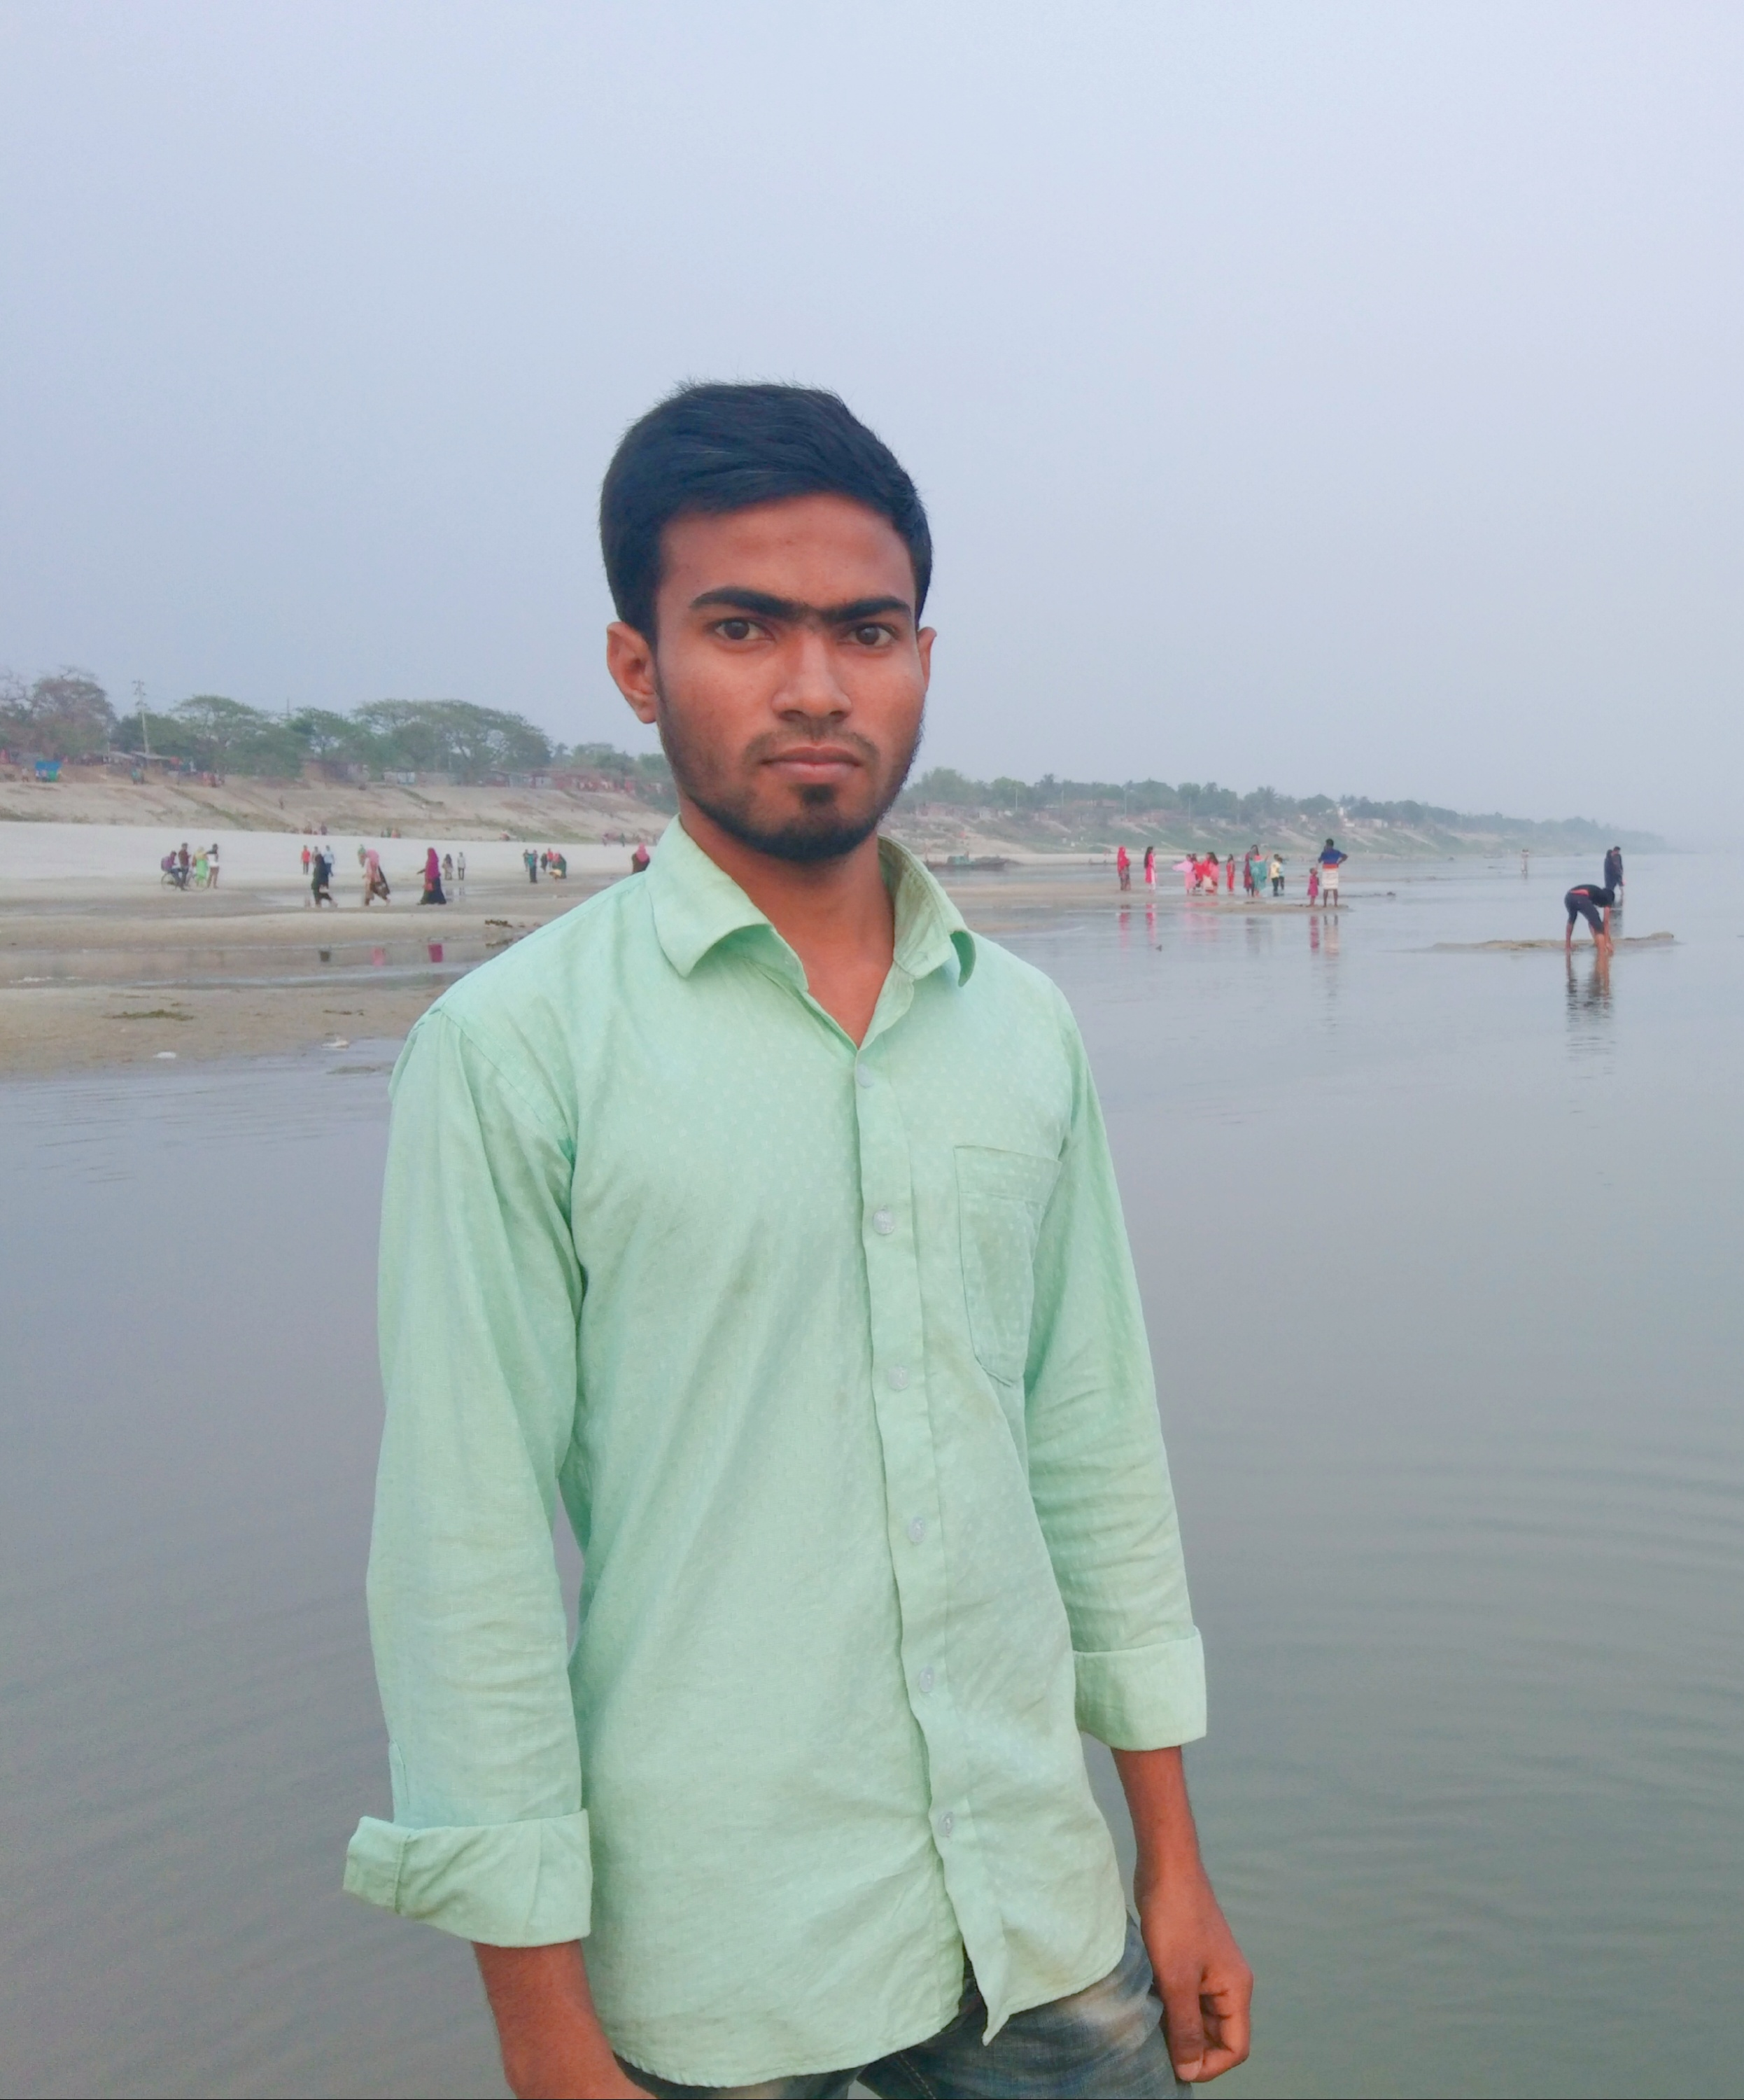
\includegraphics[width = 0.4\textwidth]{rakib.jpg}
    \caption{My picture}
    \label{fig:a}
\end{figure}
After completing my HSC exam in 2019, I prepared myself for Admission test. And finally I got a chance to admit myself in Rajshahi University. Now I live in Rajshahi. I am a second-year engineering student of Computer science and Engineering department in Rajshahi university.
\section{My experience as a cseian}
I admitted myself in RU in December, 2019. On 1st January 2020 I came to Rajshahi. I explored the whole campus day by day. Since I was a new, I felt better to see academic buildings and beautiful places. On  20 January 2020 first year first semester class started.    
\subsection{First year experience}
I was so excited in the first day of my academic class. I can not explain my feelings in words in that day. In that day I had an oriented class. So in the morning of the day I got ready for going to oriented class. After reaching our Academic building, I was excited. Our academic building is so much beautiful. Our department is located northern block of the building. As I was new I did not know where our oriented class would be held. So I asked in office about it. Then I could know that our oriented class would be held on third floor 318 no. room. After reaching on third floor, I saw my class mates stood on the portico. I went there and met with them. when it was 9 : 30 am ,then we enter for the first time in our class room.  The room was well-decorated. we gave and took our indentities with one another. After sometimes our teachers came into the room and welcome us with roses. They talk with us. From this day first year first semester class started. I attended class regularly. I was also excited in the first day of computer lab class and Basic electronics lab class. I enjoyed in lab class. I continued my class day by day. On 21th February 2020 our department made a rally for offering Flowers to central Shaheed Minar. I participated in that program. Our courses almost completed in March. Besides my academic classes , I learned programming language c++. On 18 march our campus was closed because of corona virus infection. In the time of corona pandemic, Some teachers took online class. Iqbal Aziz Khan sir gave us an assignment of game project group wise. Our group made a game named Airplane Decimating. The campus was opened again after a year later in 2021. Then our First year first semester exam date was fixed. I attended the exam. unfortunately I did not do well in the exam. After first semester exam, I prepared myself for second semester. I took some books from seminary library. In second semester I had a course named object oriented programming (java). There were two labs in the semester. Introduction to Digital System and object oriented lab. Every subject of that semester was interesting. I studied well . I completed a project named Calculator using Java. After completing our courses second semester exam date was fixed. I attended in the exam. In first semester  exam I got CGPA 3.238 and second semester exam I got CGPA 3.728. In avarage I got CGPA 3.468.
\subsection{Second year experience}
My second year first semester class was stared in march 2022. In this semester I learned data structure. Aarray, pointer, record, postfix notation, graph, tree etc were taught. Another subject is professional code writing. In this course I learned about git, github, and professional code writing. Theory of statistics, math, digital system design, discrete math etc were taught. I also learned Management and Accountance. I took some books for that course from seminary library. Besides my academic studies, I have learned basic python language, basic javascript. At the end of the course, I completed my 1st semester exam. I started my second semester 2nd year class.     
\section{Conclusion}
There is no limit of gaining experiences. I have gained some experiences in 3 semesters. I have to learn more and more. After completing this semester I will learn about Technical writing, Algorithms, Computer Architecture and Organization, Web Application Development.  
\end{document}
